\documentclass{beamer}
\usetheme{Frankfurt} 
\usecolortheme{whale}
\usepackage{graphicx}
\graphicspath{ {./images/} }


\title{Parallel Game Tree Search: Gomoku}
\author[My name]{Yuya Kawakami \& Haoran Wang}
\date{Dec 3, 2020}

%\usetheme{lucid}
\begin{document}
	\frame {
		\titlepage
	}

	\frame{
		\frametitle{Introduction}
		\framesubtitle{Gomoku}
			\begin{itemize}
				\item Also called Five in a Row.
				\item More complex and difficult than Tic Tac Toe.
			\end{itemize}
			\medskip
			\begin{figure}[!htbp]
				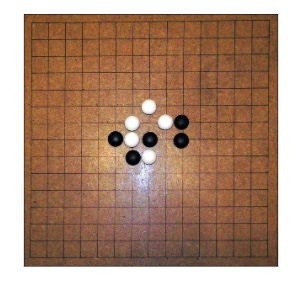
\includegraphics[scale=0.5]{img1}
			\end{figure}
	}

	\frame {
		\frametitle{Introduction}
		\framesubtitle{Minimax Game Tree for Zero-Sum Game}
			\begin{itemize}
				\item Maximizer tries to get the highest score.
				\item Minimizer tries to get the lowest score.
			\end{itemize}
	
			\begin{figure}[!htbp]
				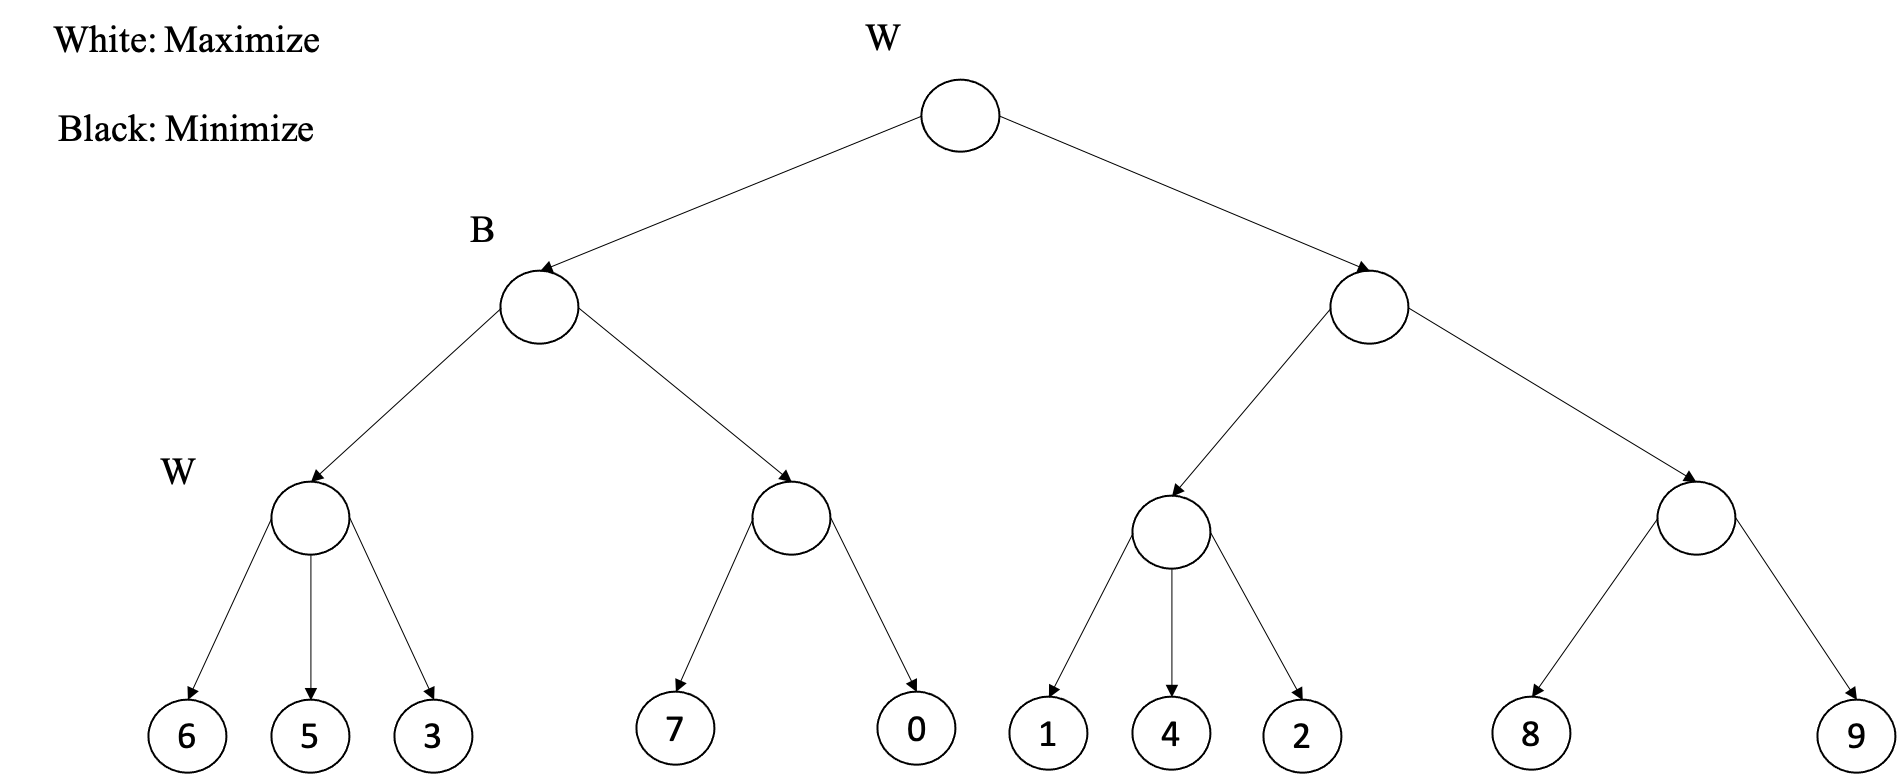
\includegraphics[scale=0.35]{img2}
			\end{figure}
	}
	
	\frame {
		\frametitle{Introduction}
		\framesubtitle{Minimax Game Tree for Zero-Sum Game}
		
		\begin{figure}[!htbp]
			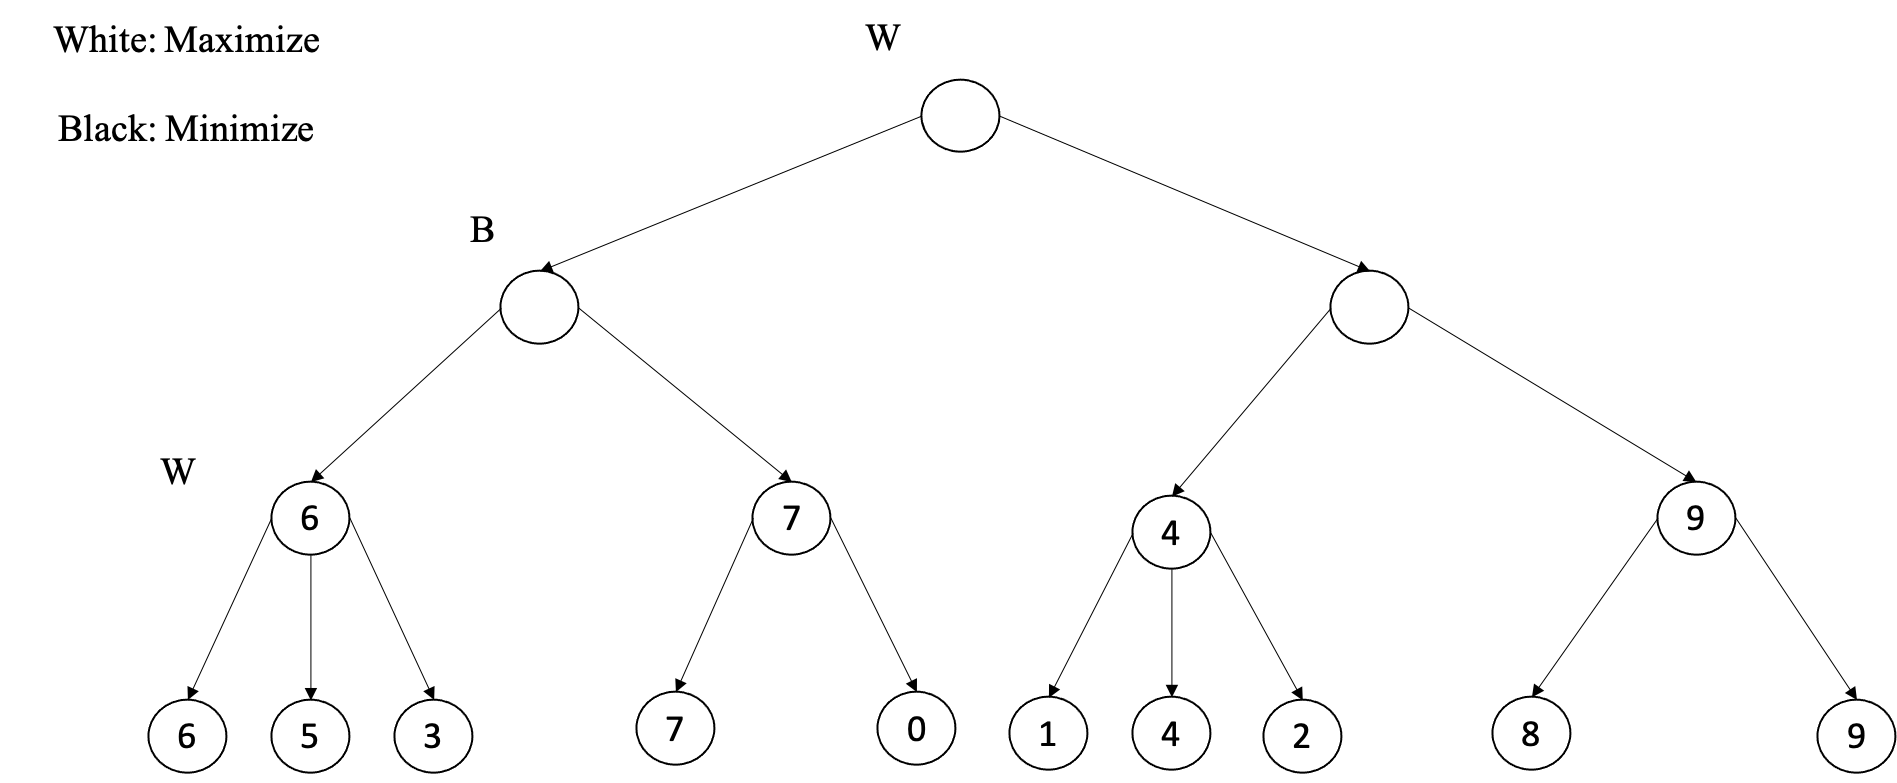
\includegraphics[scale=0.35]{img3}
		\end{figure}
	}
	
	\frame {
		\frametitle{Introduction}
		\framesubtitle{Minimax Game Tree for Zero-Sum Game}
		
		\begin{figure}[!htbp]
			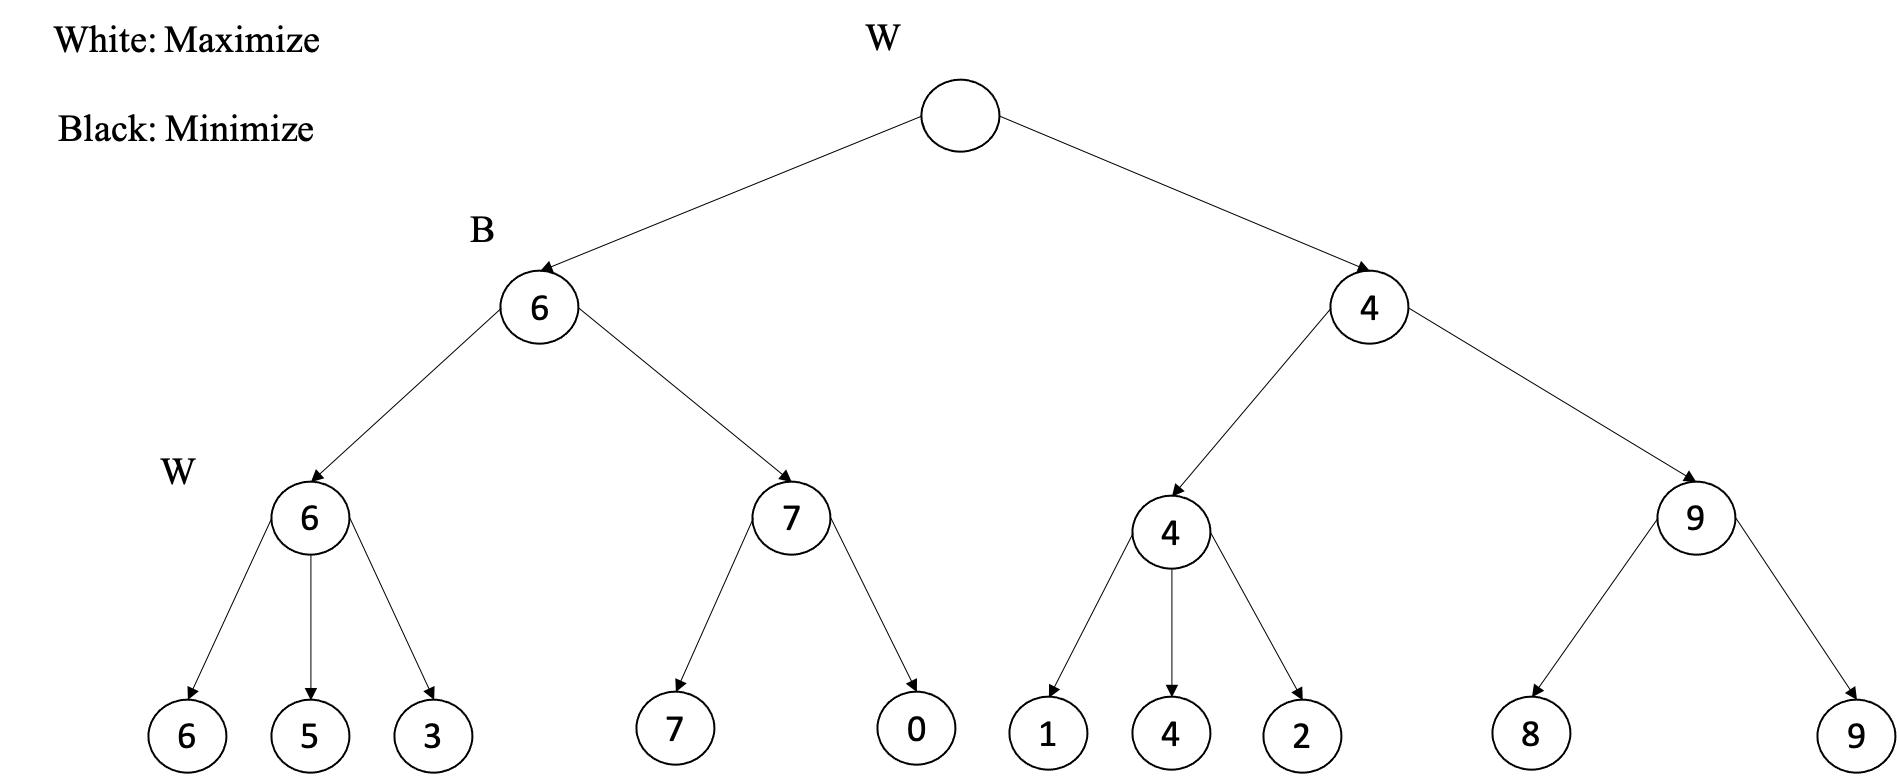
\includegraphics[scale=0.35]{img4}
		\end{figure}
	}
	
	\frame {
		\frametitle{Introduction}
		\framesubtitle{Minimax Game Tree for Zero-Sum Game}
		
		\begin{figure}[!htbp]
			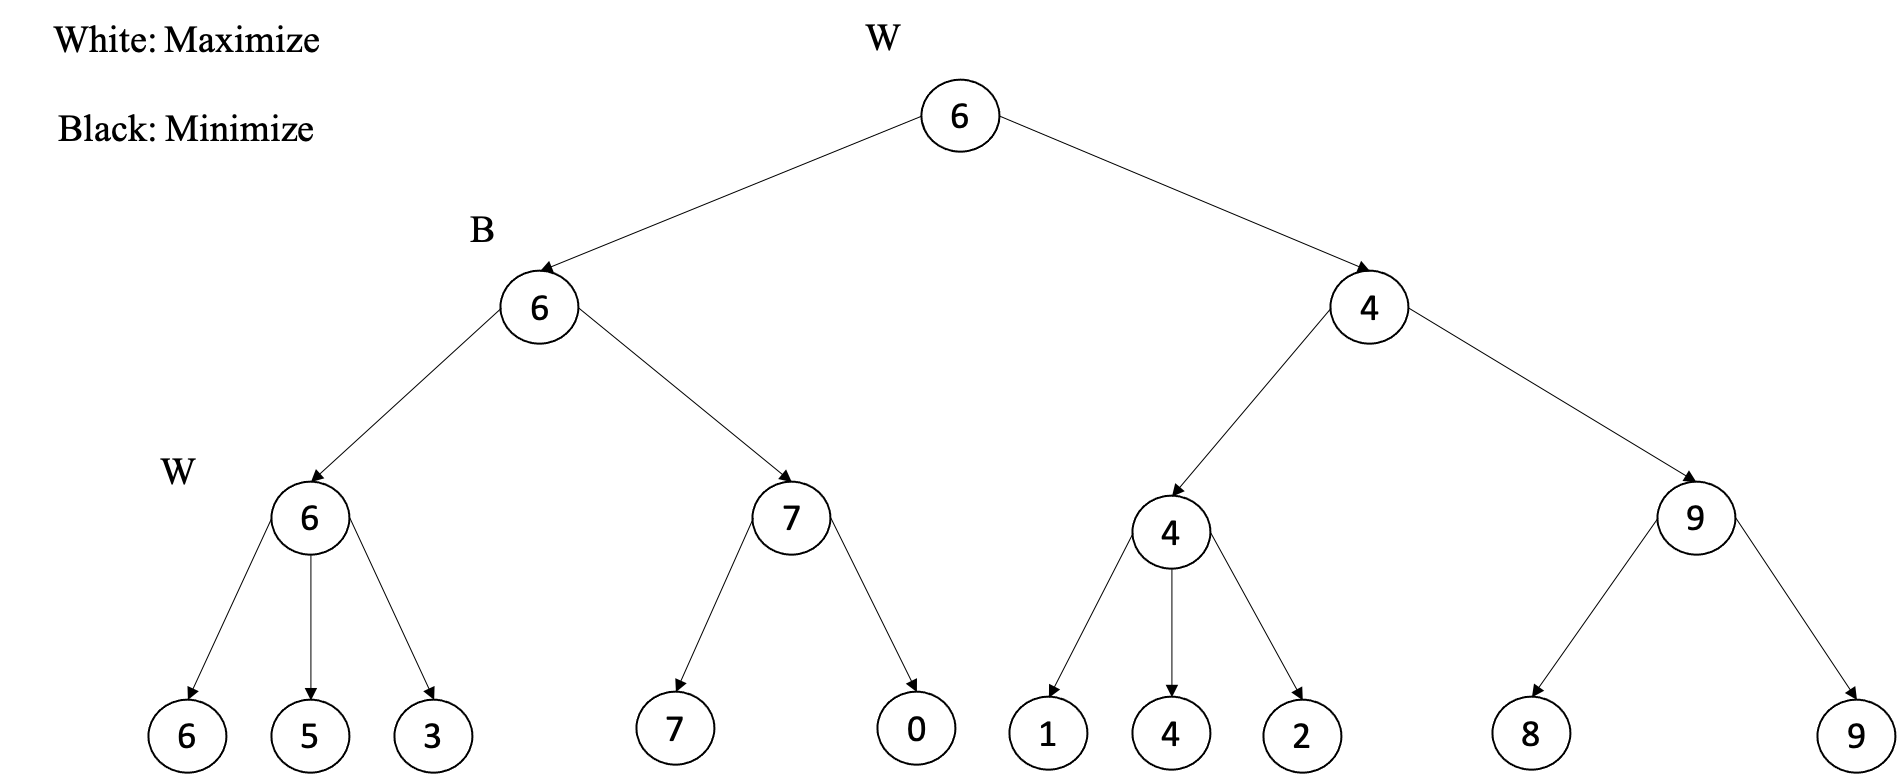
\includegraphics[scale=0.35]{img5}
		\end{figure}
	}
	
	\frame {
		\frametitle{Introduction}
		\framesubtitle{Alpha-Beta Pruning}
		\begin{itemize}
			\item Alpha: It is the lower bound of possible solutions for maximizer.
			\item Beta: It is the upper bound of possible solutions for minimizer.
		\end{itemize}
	}

	\frame {
		\frametitle{Introduction}
		\framesubtitle{Alpha-Beta Pruning}
		\begin{itemize}
			\item If beta <= alpha is true, we can prune.
		\end{itemize}
		
		\begin{figure}[!htbp]
			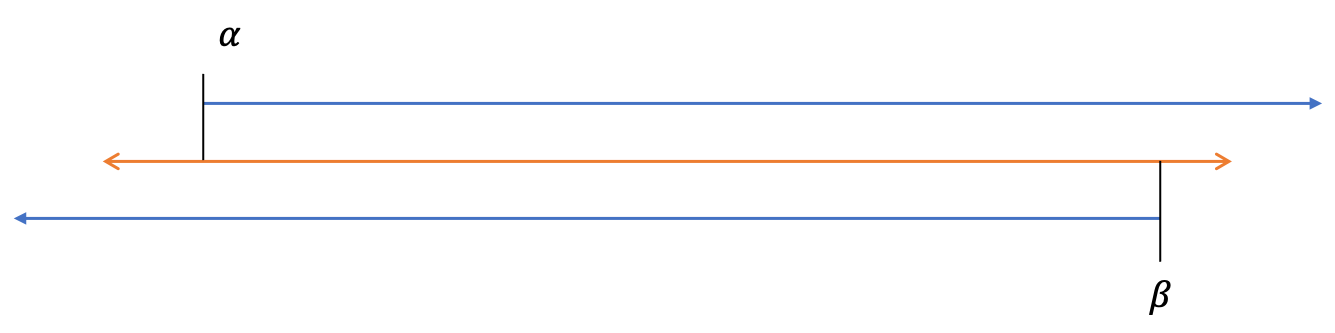
\includegraphics[scale=0.35]{img6}
		\end{figure}
		
		\begin{figure}[!htbp]
			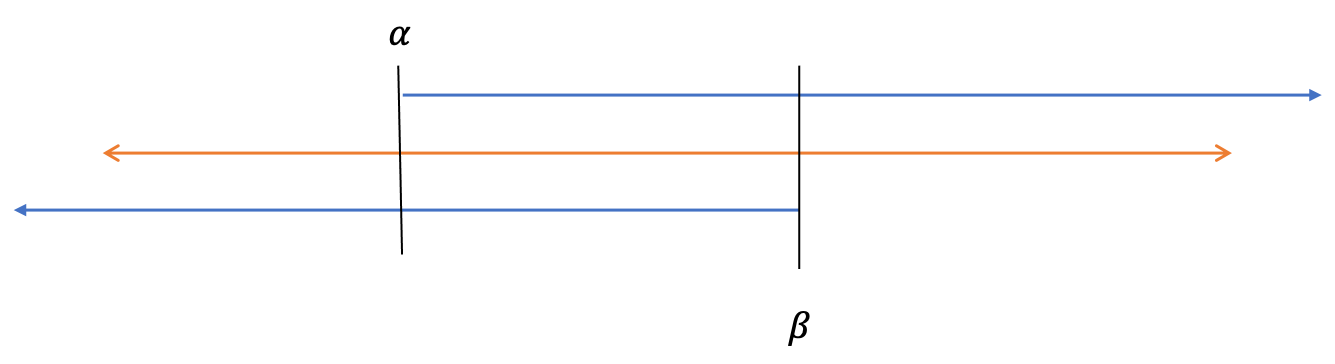
\includegraphics[scale=0.35]{img7}
		\end{figure}
		
		\begin{figure}[!htbp]
			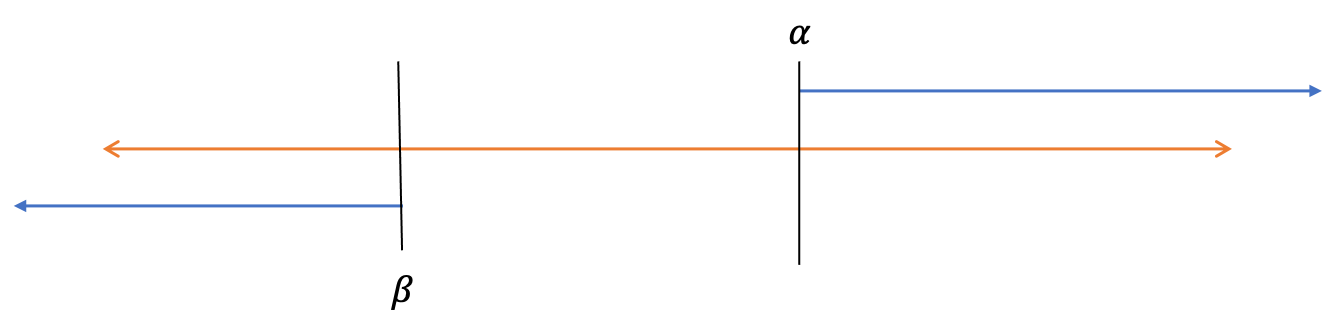
\includegraphics[scale=0.35]{img8}
		\end{figure}
	}
	
	\frame {
		\frametitle{Introduction}
		\framesubtitle{Alpha-Beta Pruning}
		
		\begin{figure}[!htbp]
			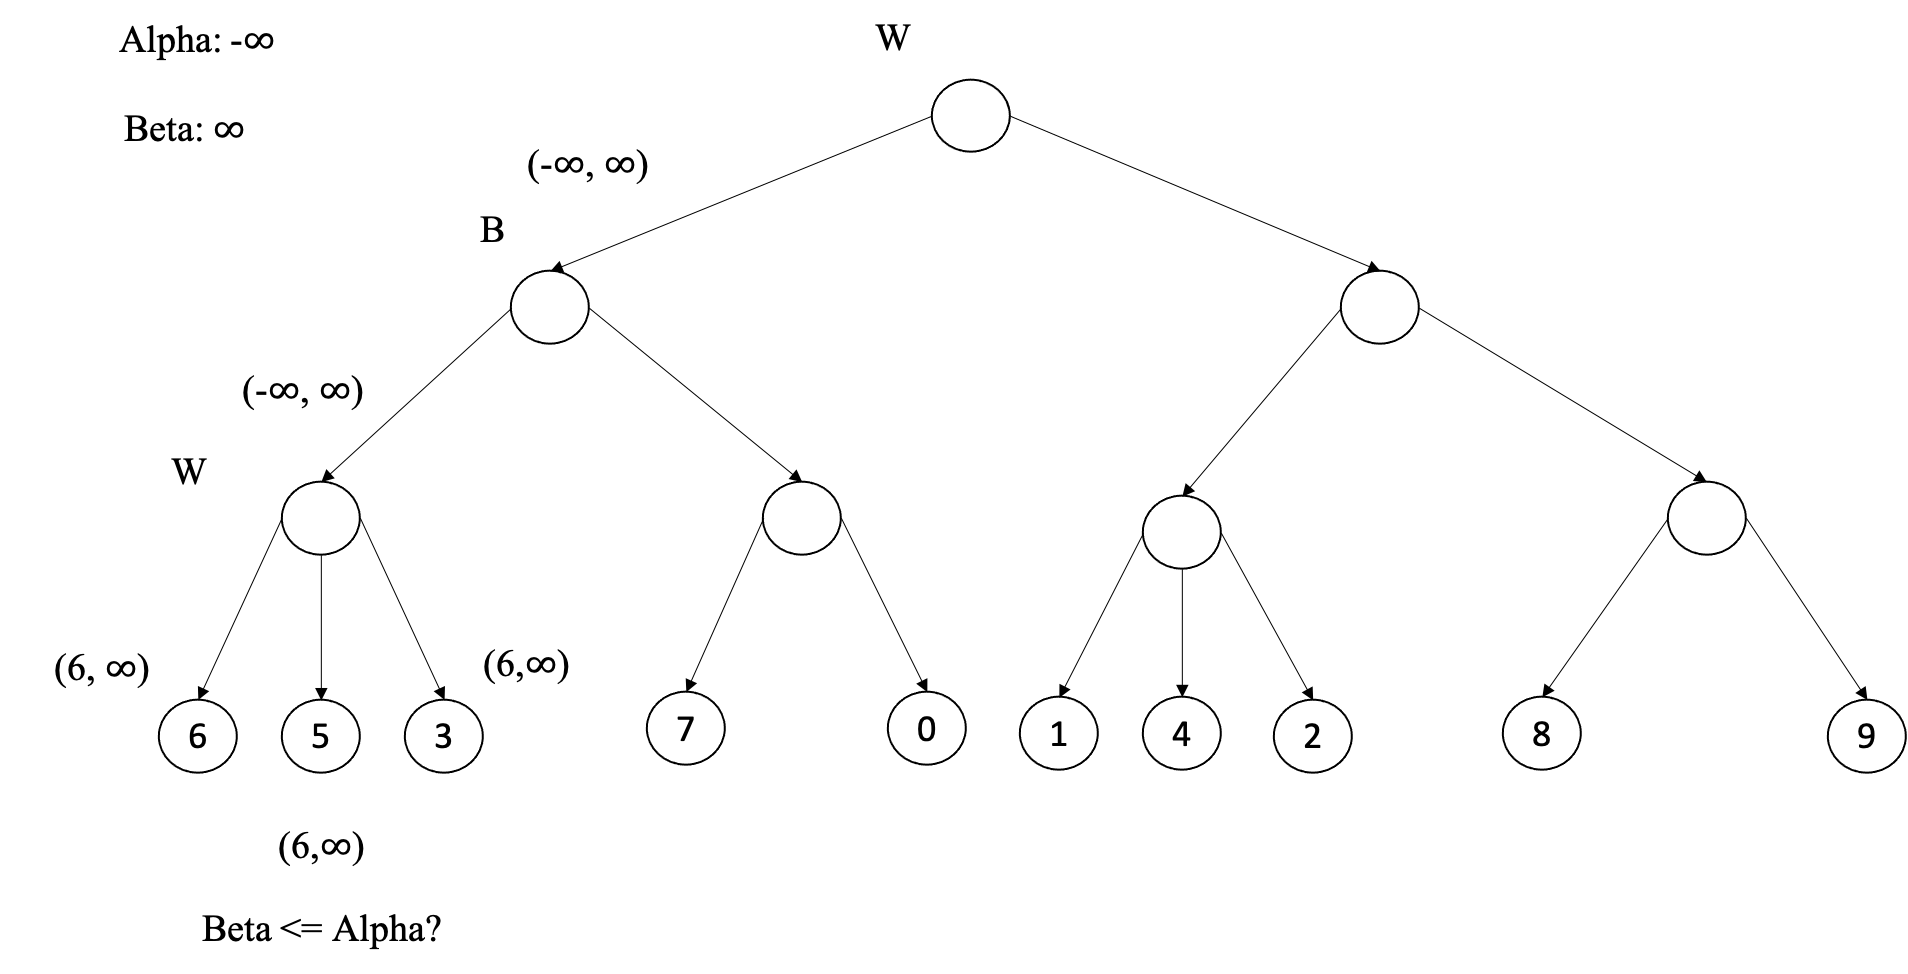
\includegraphics[scale=0.35]{img9}
		\end{figure}
	}

	\frame {
		\frametitle{Introduction}
		\framesubtitle{Alpha-Beta Pruning}
		
		\begin{figure}[!htbp]
			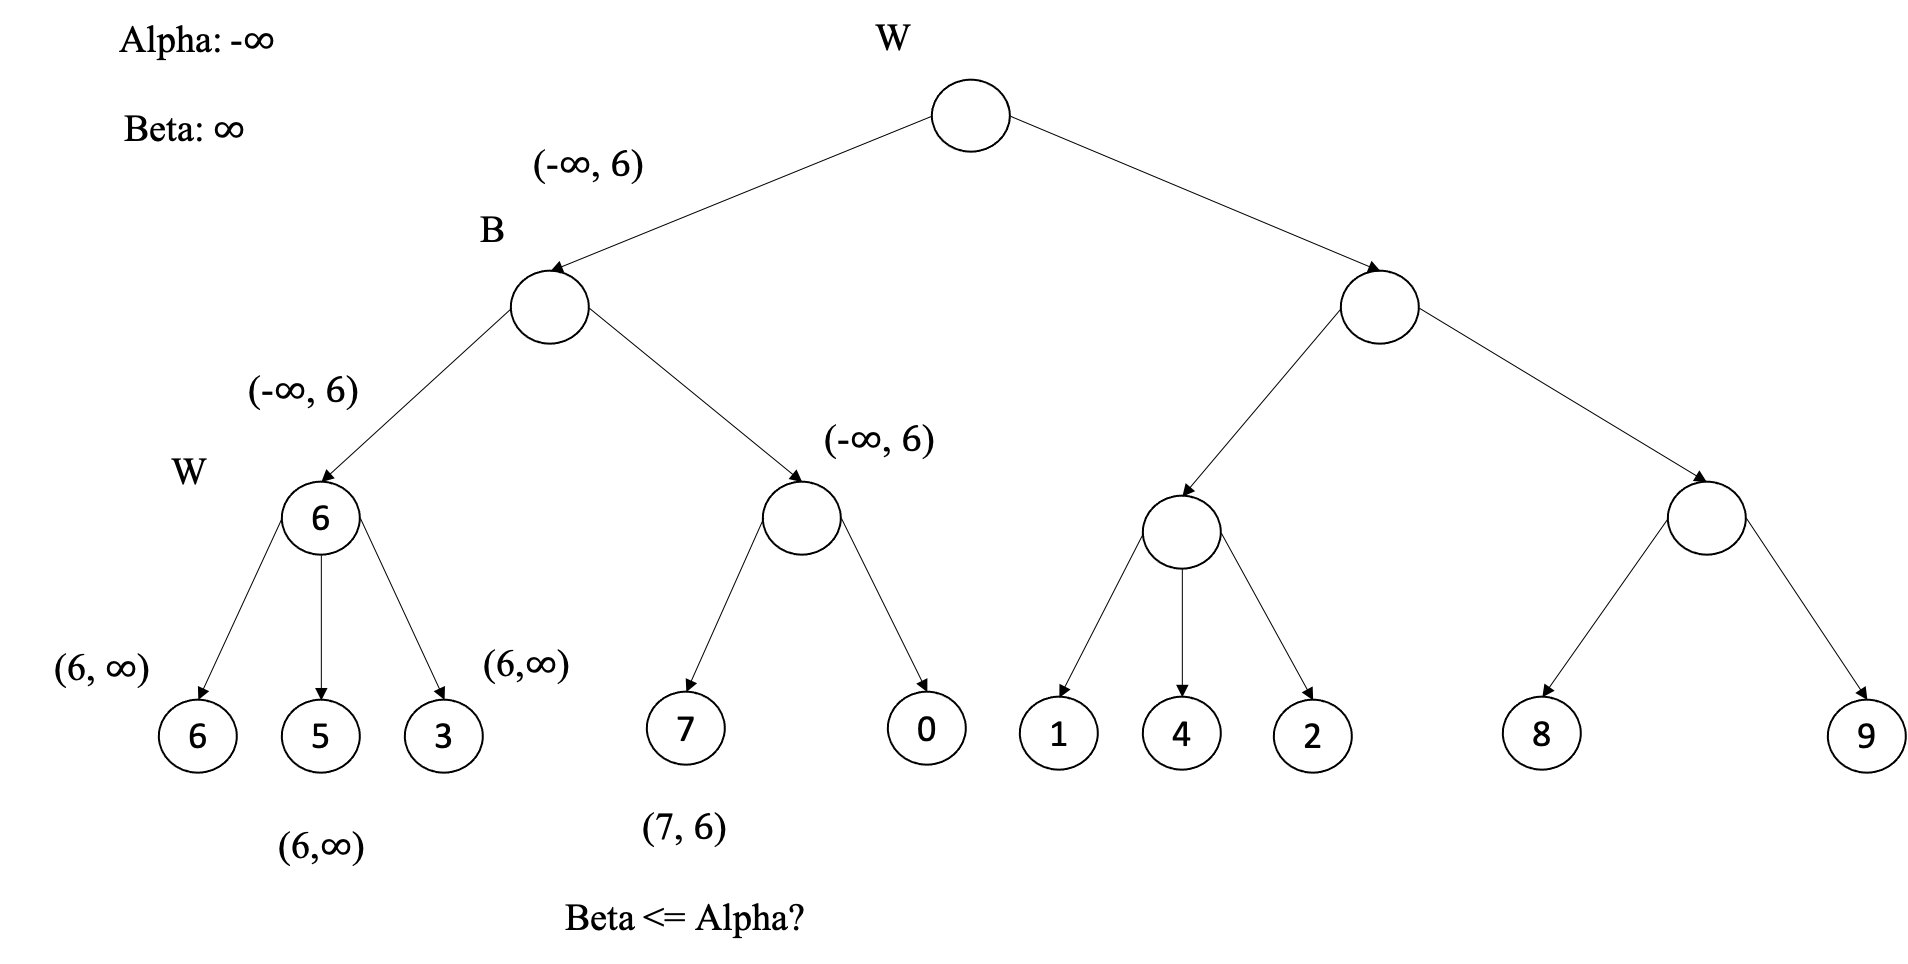
\includegraphics[scale=0.35]{img10}
		\end{figure}
	}
	
	\frame {
		\frametitle{Introduction}
		\framesubtitle{Alpha-Beta Pruning}
		
		\begin{figure}[!htbp]
			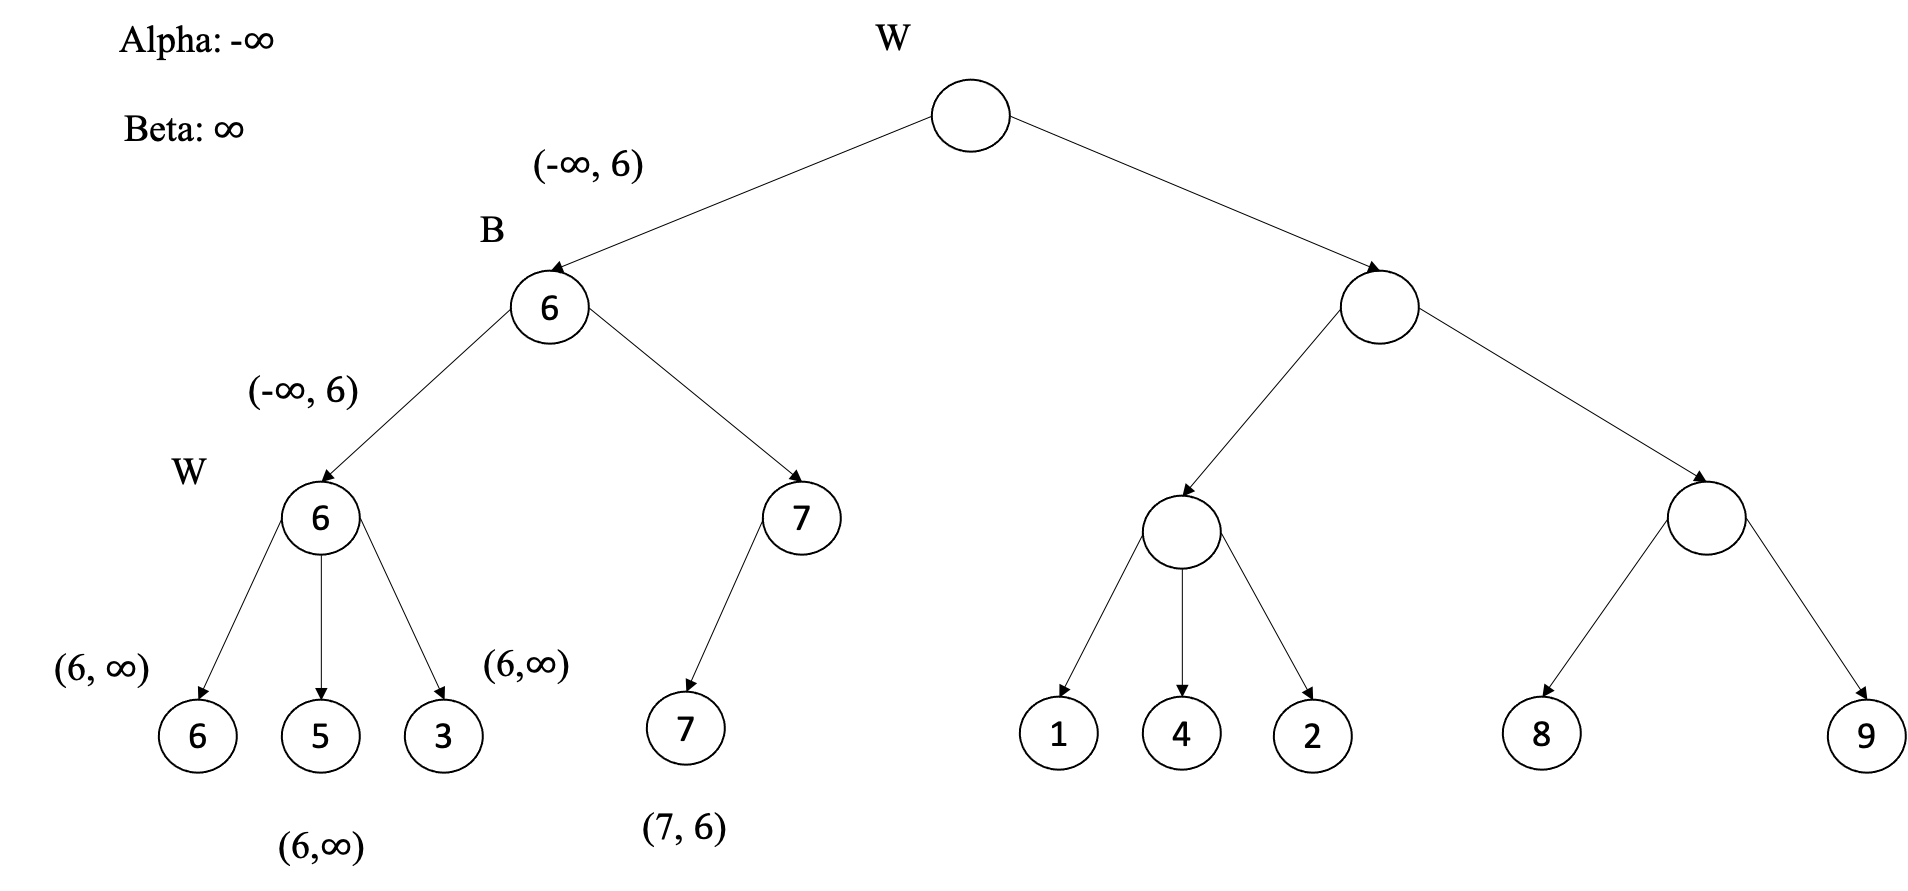
\includegraphics[scale=0.35]{img11}
		\end{figure}
	}
	
	\frame {
		\frametitle{Introduction}
		\framesubtitle{Heuristic: Stone Shapes}
		\begin{itemize}
			\item Five in a Row
			\item Live Four
			\item Dead Four
			\item Live Three
			\item Dead Three
			\item Live Two
			\item Dead Two
		\end{itemize}
	}
	
	\frame {
		\frametitle{Introduction}
		\framesubtitle{Heuristic: Stone Shapes}
		\begin{figure}[!htbp]
			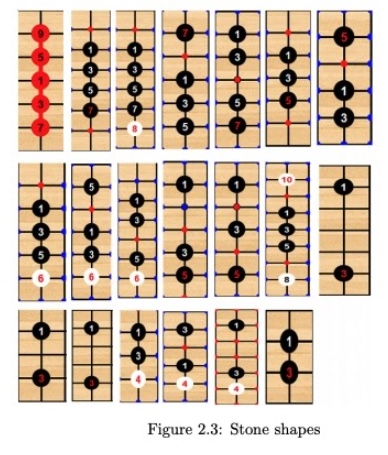
\includegraphics[scale=0.4]{img12}
		\end{figure}
	}
	
	\frame {
		\frametitle{Solutions}
		\framesubtitle{OpenMP}
		\begin{itemize}
			\item Since the tree search is called recursively, OpenMP is trivial.
			\item Even with OpenMP, CPU has limited capability of searching at a higher depth on a larger board.
		\end{itemize}
	}
	
	\frame {
		\frametitle{Solutions}
		\framesubtitle{Naive CUDA}
		\begin{itemize}
			\item Launch a GPU thread for each possible move from the root node.
			\item Introduces thread divergence -> very poor performance.
			\item A lot of work for little number of threads.
		\end{itemize}
		\begin{figure}[!htbp]
			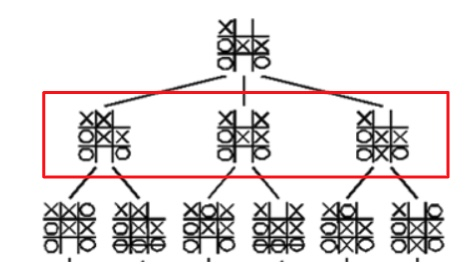
\includegraphics[scale=0.4]{img13}
		\end{figure}
	}

	\frame {
		\frametitle{Solutions}
		\framesubtitle{Sequential-Parallel CUDA implementation}
		\begin{itemize}
			\item Idea: Launch as many light weight GPU threads.
			\item Process some depth s on the CPU and get k leaf nodes.
			\item Calculate these k leaf nodes in parallel.
		\end{itemize}
		\begin{figure}[!htbp]
			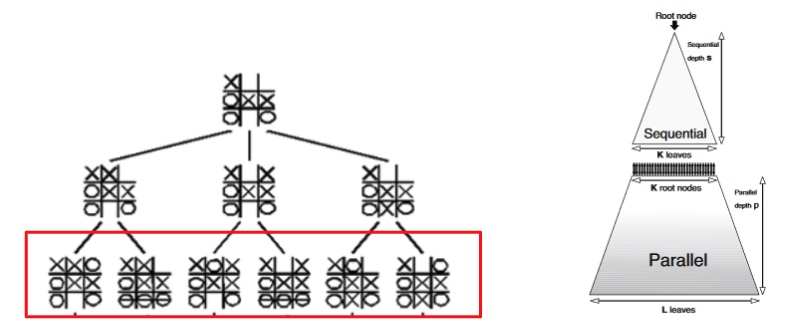
\includegraphics[scale=0.4]{img14}
		\end{figure}
	}
	
	\frame {
		\frametitle{Solutions}
		\framesubtitle{Problems with Naive CUDA implementation}
		\begin{itemize}
			\item The result from earlier branches are used to determine whether later branches should be examined or not.
			\item If we search multiple branches in parallel, those branches do not have the bounds from each other to work with.
			\item This will result in searching branches that would have been pruned in the serialized version.
			\item In theory, a thread searching one branch could update the other threads with its bounds when the thread finishes.
			\item However, it is difficult to implement on GPU since it would require blocks to be able to break other blocks out of recursive function calls.
		\end{itemize}
	}
	
	\frame {
		\frametitle{Solutions}
		\framesubtitle{PVS: Principle Variation Search}
		\begin{itemize}
			\item Idea: Search down the leftmost branch of the tree on CPU, and then search the remaining nodes in parallel on GPU.
			\item This allows the GPU branches to use the bounds from the first CPU-searched branch.
		\end{itemize}
		\begin{figure}[!htbp]
			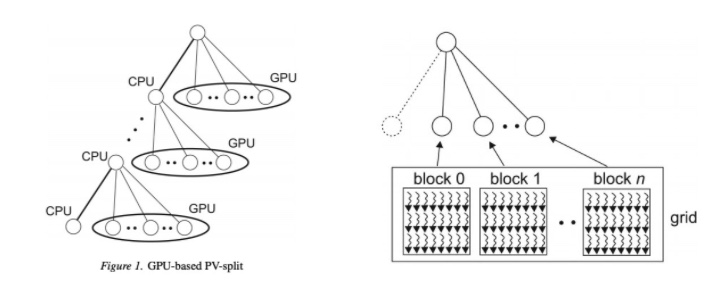
\includegraphics[scale=0.4]{img15}
		\end{figure}
	}
	
	\frame {
		\frametitle{Solutions}
		\framesubtitle{PVS: Principle Variation Search}
		\begin{itemize}
			\item One block per child node.
			\item Use that block to search down the subtree rooted at the child node.
			\item As depth increasing, GPU threads need to search increasingly larger subtrees.
			\item Even though there are many threads searching in parallel, each thread has to search a subtree serially.
			\item Therefore, we can further parallelize subtree searching.
		\end{itemize}
	}
	
	\frame {
		\frametitle{Solutions}
		\framesubtitle{Dynamic Parallelism}
		\begin{itemize}
			\item Launch a new kernel for each node to searched, instead of using one block to fully search a subtree.
			\item The overall structure remains the same. CPU will search one branch of the tree, and using the bounds obtained for GPU to search the remaining nodes.
			\item One possible trade off is the overhead of launching so many kernels.
		\end{itemize}
	}

	\frame {
		\frametitle{Experiments}
		\framesubtitle{Performance to Calculate One Step}
		\begin{figure}[!htbp]
			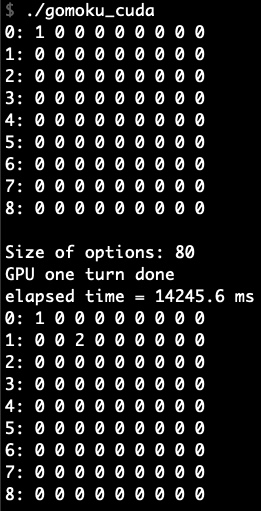
\includegraphics[scale=0.38]{img18}
		\end{figure}
	}
	
	\frame {
		\frametitle{Results}
		\framesubtitle{Depth = 3}
		Time measured in seconds.
		\begin{figure}[!htbp]
			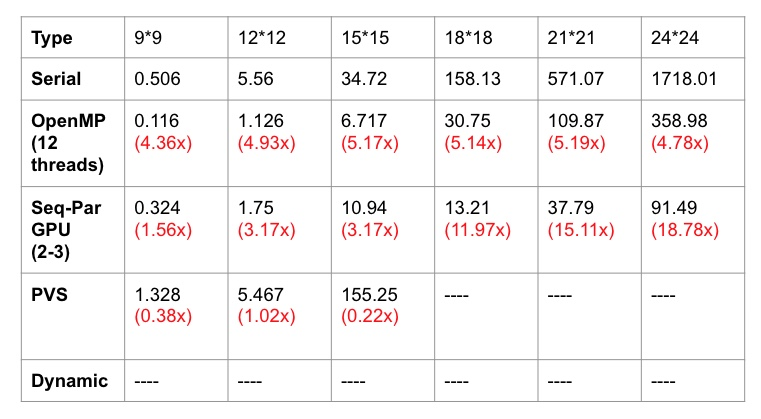
\includegraphics[scale=0.38]{img16}
		\end{figure}
	}
	
	\frame {
		\frametitle{Observation}
		\framesubtitle{Depth = 3}
		\begin{itemize}
			\item OpenMP achieved steady speedup when the board size grows.
			\item Seq-Par achieved very good speedup when the board size grows.
			\item PVS suffered when the board size grows.
			\item Dynamic took too long to finish at this depth.
		\end{itemize}
	}

	\frame {
		\frametitle{Results}
		\framesubtitle{Depth = 4}
		Time measured in seconds.
		\begin{figure}[!htbp]
			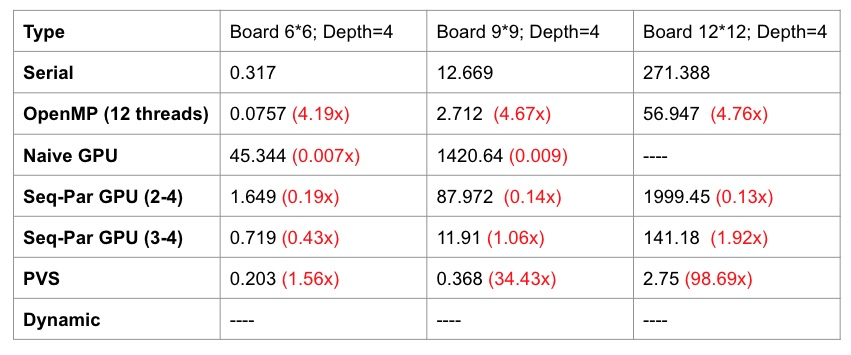
\includegraphics[scale=0.35]{img17}
		\end{figure}
	}
	
	\frame {
		\frametitle{Observation}
		\framesubtitle{Depth = 4}
		\begin{itemize}
			\item OpenMP achieved steady speedup when the board size grows.
			\item Naive GPU suffered when the board size grows.
			\item Seq-Par achieved very little speedup  when the board size grows.
			\item PVS achieved impressive speedup when the board size grows.
			\item Dynamic took too long to finish at this depth.
		\end{itemize}
	}
	
	\frame {
		\frametitle{Experiments}
		\framesubtitle{Performance to Calculate a Whole Game}
		\begin{figure}[!htbp]
			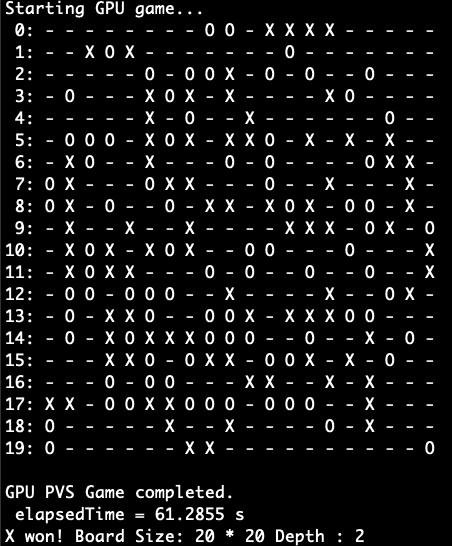
\includegraphics[scale=0.38]{img19}
		\end{figure}
	}

	\frame {
		\frametitle{Results}
		\framesubtitle{}
		\begin{figure}[!htbp]
			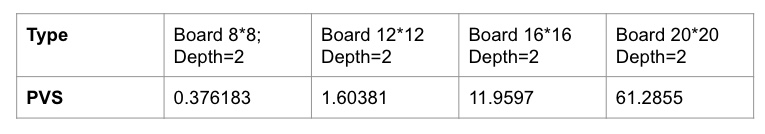
\includegraphics[scale=0.38]{img20}
		\end{figure}
		
		Our PVS and Dynamic implementation was fixed at the last minute. We will include the experiment results in final report.
	}

	\frame {
		\frametitle{Citation}
		\framesubtitle{}
		\begin{itemize}
			\item D. Strnad and N. Guid, "Parallel alpha-beta algorithm on the GPU," CIT, vol. 19, no. 4,pp. 269-274, 2011.
			\item K. Rocki and R. Suda, "Parallel Minimax Tree Searching on GPU", JST CREST, 2009.
			\item Li, L., Liu, H., Wang, H., Liu, T., Li, W.: A parallel algorithm for game tree search
			using gpgpu (2014)
			\item H. Liao, "New Heuristic algorithm to improve the Minimax for Gomoku artificial intelligence.", 2019.
			\item Marsland, T.A., Campbell, M.: Parallel search of strongly ordered game trees.
			ACM Computing Surveys (CSUR) 14(4), 533–551 (1982)
			\item Strnad, D., Guid, N.: Parallel alpha-beta algorithm on the gpu. In: Information
			Technology Interfaces (ITI), Proceedings of the ITI 2011 33rd International Conference on. pp. 571–576. IEEE (2011)
		\end{itemize}
	}
	
	\frame {
		\frametitle{Conclusion}
		\framesubtitle{Limitations and Possible Optimizations}
		Sequential-Parallel CUDA
		\begin{itemize}
			\item Needs memory optimizations for it run at higher depths and larger boards.
			\item Redundant calculations.
		\end{itemize}
	}
	
	\frame {
		\frametitle{Questions?}
		\framesubtitle{}
		Thank you!
	}
	
\end{document}